\documentclass[main]{subfiles}
\begin{document}

%@@@@@@@@@@@@@@@@@@@@@@@@@@@@@@
% Main Topics: Perceptron Learning Algorithm 06.12.2018
% Lecturer: Matthew Cook
% author: Vanessa Leite - base document from benelot/eth-intro-to-neuroinformatics-summary

\section{Perceptron}

\subsection{Converting real weights to integer}
Any unit can be converted into one with integer weights.

\begin{figure}[H]
	\centering
	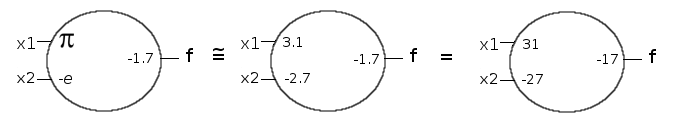
\includegraphics[width=0.8\textwidth]{converting-units-integer.png}
	\caption{Converting real weights to integer}
	\label{fig:converting}
\end{figure}

Figure~\ref{fig:converting} shows the approach to convert real weights to integer. The approximation (images left and center) can be problematic if $x$ in $\theta(x)$ is equal to zero (in the real setup), because it can be shifted in the approximation.
In the second step (images center and right) there is no problem. By multiplying the weights per a factor of 10, we do not change the value of $x$ in $\theta(x)$.

One way to solve the above problem (approximation) is to shift the bias term a bit.

\begin{enumerate}
\item Find the largest possible negative sum (closest to zero)
\item Adjust bias (increase) if necessary so no sum is zero
\item Replace weights with rational approximations more precise than sum closest to zero
\item Scale up weights to be integers
\end{enumerate}

In the first two steps, we avoid have a sum of zero. On the last two, we transform the weights to integer.

So far, the difference of this unit and a real neuron is that neurons can adjust their own weight (learning) and these units are behaving as gates.

\end{document}
